\section{General setup}\label{sec:general-setup}
GRATiS uses GROOVE as a replacement of the IOSTS in ATM. Figure~\ref{fig:tooling} shows the collaboration diagram of GRATiS. GROOVE has several exploration strategies for exploring a GG to a GTS. The SymbolicStrategy is added as exploration strategy. It contains functionality to build an STS from a GG. The STS is sent as a JSON message by the GrooveInterface to a remote host. The ATMInterface receives the message and starts the test run.

\begin{figure}[ht]
  \begin{center}
    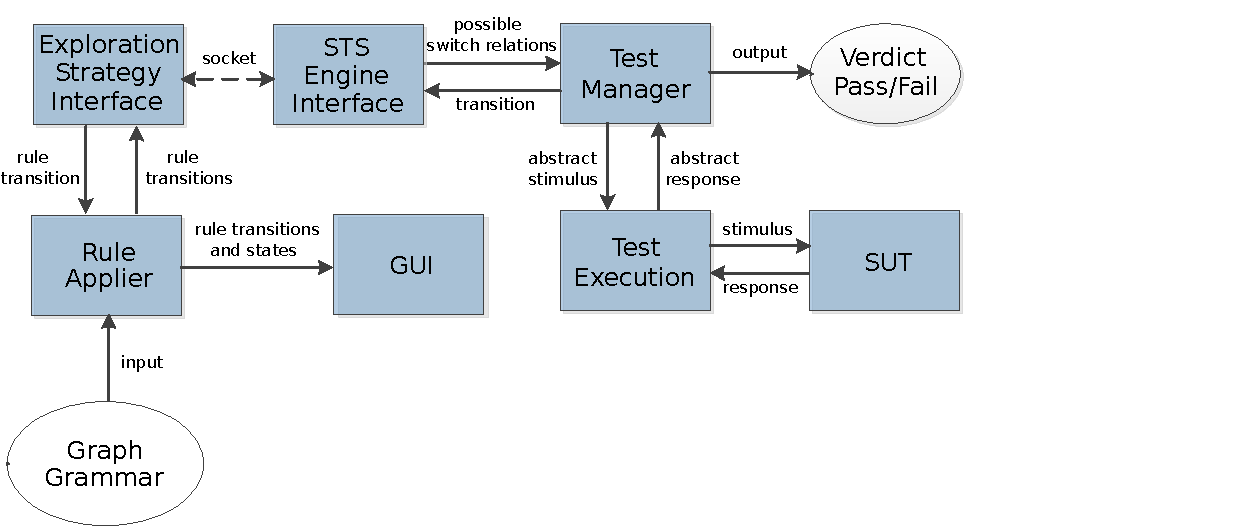
\includegraphics[width=\textwidth]{tooling.pdf}
  \end{center}
  \caption{GRATiS collaboration diagram}
  \label{fig:tooling}
\end{figure}\marginpar{change into sequence diagram VISIO. What to use as static diagram?? UML. Should User be modelled? Not with sequence}

\section{Description of added functionality}
This section covers in detail the added functionality to GROOVE and ATM. 

\subsection{GROOVE exploration strategy}
Figure~\ref{fig:esi-diagram} shows the class diagram of the added exploration strategy interface. The symbolic exploration strategy has an exploration strategy such as the Breadth-First exploration strategy to explore the GTS. The remote exploration strategy extends the symbolic exploration strategy.

The user starts the remote exploration strategy. This strategy starts a Breadth-First exploration strategy. This strategy explores the GTS and notifies the remote strategy when there are no more rule transitions to explore. The symbolic strategy builds the STS in Java objects using the explored rule transitions. The class diagram  of the STS is given in section~\ref{sec:sts-setup}. The remote strategy sends the STS in JSON format as a HTTP PUT request to the interface at ATM.\marginpar{need to say more about the way GROOVE does exploration. Here or in tooling? Where does point algebra come in?}

The Breadth-First exploration strategy and the symbolic strategy are loosely coupled, such that other strategies can also be used if desired.
 
\begin{figure}[ht]
  \begin{center}
    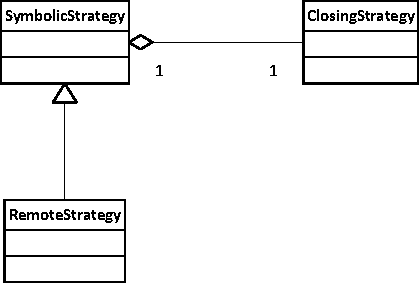
\includegraphics[width=0.35\textwidth]{strategy.pdf}
  \end{center}
  \caption{The class diagram of the exploration strategy interface}
  \label{fig:esi-diagram}
\end{figure}

\subsection{STSs}\label{sec:sts-setup}
Figure~\ref{fig:sts-diagram} shows the class diagram of the STS in GRATiS. The STS is composed of Locations, Switch relations, Gates, Interaction and Location variables. A Location can be the start and target of any number of switch relations. A switch relation has two locations; the start and target location. A Switch relation has one gate and a gate can belong to any number of switch relations. A gate can have any number of interaction variables, but an interaction variable belongs to one gate. The STS has a singleton class, the RuleInspector, which contains the functionality of building guards and updates from rule graphs.\marginpar{discuss correspondence to small model}

\begin{figure}[ht]
  \begin{center}
    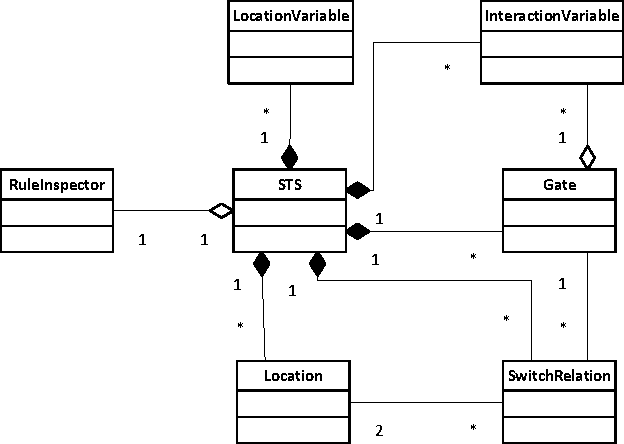
\includegraphics[width=0.5\textwidth]{STS.pdf}
  \end{center}
  \caption{The class diagram of the STS in GRATiS}
  \label{fig:sts-diagram}
\end{figure}

\subsection{ATM Interface}
The ATM interface is one component in the Rails framework. It receives the STS request\marginpar{how?}, builds the STS as Ruby objects and initiates the test run using this STS as model.